\documentclass{article}
\usepackage{graphicx}
\usepackage{hyperref}
\usepackage{amsmath}
\usepackage{times}

\textwidth=6.2in
\textheight=8.5in
%\parskip=.3cm
\oddsidemargin=.1in
\evensidemargin=.1in
\headheight=-.3in


%------------------------------------------------------------
% newcommand
%------------------------------------------------------------
\newcommand{\scscst}{\scriptscriptstyle}
\newcommand{\scst}{\scriptstyle}
\newcommand{\Robject}[1]{{\texttt{#1}}}
\newcommand{\Rfunction}[1]{{\texttt{#1}}}
\newcommand{\Rclass}[1]{\textit{#1}}
\newcommand{\Rpackage}[1]{\textit{#1}}
\newcommand{\Rexpression}[1]{\texttt{#1}}
\newcommand{\Rmethod}[1]{{\texttt{#1}}}
\newcommand{\Rfunarg}[1]{{\texttt{#1}}}

\usepackage{Sweave}
\begin{document}
\Sconcordance{concordance:sea_lion_risk.tex:sea_lion_risk.Rnw:%
1 27 1 1 0 23 1 11 0 1 4 5 1 15 0 1 6 1 1 1 3 6 0 1 2 6 1 11 0 1 5 3 1 %
24 0 1 4 5 1 35 0 1 7 9 1}


%------------------------------------------------------------
\title{Ivermectin trial}
%------------------------------------------------------------
\author{David Hayman}
%\date{}





\maketitle
%\tableofcontents


%-------------------------------------------
\section{The sex and ivermectin effect}
%--------------------------------------------

This uses your data from the slides and the number dead and the numbers of treatments and controls. First we look at the sex effect:

\begin{Schunk}
\begin{Sinput}
> sex <- matrix(c(32, 148, 43, 119), ncol = 2)
> colnames(sex) <- c("male", "female")
> rownames(sex) <- c("died", "survive")
> print(sex)
\end{Sinput}
\begin{Soutput}
        male female
died      32     43
survive  148    119
\end{Soutput}
\begin{Sinput}
> chisq.test(sex)
\end{Sinput}
\begin{Soutput}
	Pearson's Chi-squared test with Yates' continuity correction

data:  sex
X-squared = 3.3315, df = 1, p-value = 0.06796
\end{Soutput}
\begin{Sinput}
> chisq.test(sex, simulate.p.value = T, B = 10000)
\end{Sinput}
\begin{Soutput}
	Pearson's Chi-squared test with simulated p-value (based on 10000
	replicates)

data:  sex
X-squared = 3.8264, df = NA, p-value = 0.06689
\end{Soutput}
\end{Schunk}

There seems to be no sex effect - i.e. sex is not a risk factor given these sample sizes, despite the difference in mortality and inclusion of the denominator data, i.e. how many in your study were male vs female.

Next we look at the ivermectin effect:

\begin{Schunk}
\begin{Sinput}
> ivermectin <- matrix(c(21, 142, 41, 137), ncol = 2)
> chisq.test(ivermectin)
\end{Sinput}
\begin{Soutput}
	Pearson's Chi-squared test with Yates' continuity correction

data:  ivermectin
X-squared = 5.2302, df = 1, p-value = 0.0222
\end{Soutput}
\begin{Sinput}
> rownames(ivermectin) <- c("died", "survive")
> colnames(ivermectin) <- c("ivermectin", "control")
\end{Sinput}
\end{Schunk}

\begin{figure}
\begin{Schunk}
\begin{Sinput}
> barplot(ivermectin,legend=T,beside=T,main='Ivermectin control',
+          args.legend = list(x = "topright", bty = "n", inset=c(0.3, 0.1)))
\end{Sinput}
\end{Schunk}
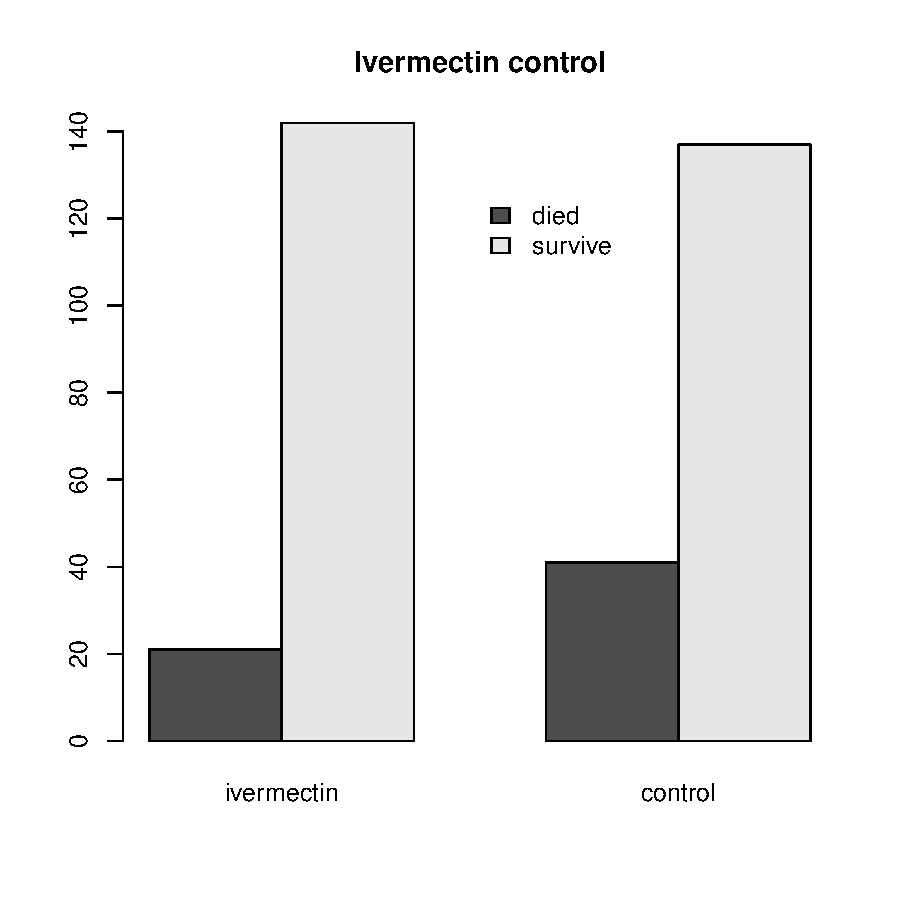
\includegraphics{Fig-test3}
\caption{Cohort study data}
\label{fig:p}
\end{figure}

We can estimate the relative risk etc by using the 2 * 2 table, e.g.:

\begin{Schunk}
\begin{Sinput}
> rel.risk <- (ivermectin[1, 1]/sum(ivermectin[1, ]))/(ivermectin[2, 
+     1]/sum(ivermectin[2, ]))
> abs.risk.reduction <- (ivermectin[1, 1]/sum(ivermectin[, 1]))/(ivermectin[1, 
+     2]/sum(ivermectin[, 2]))
> abs.risk.reduction
\end{Sinput}
\begin{Soutput}
[1] 0.5593296
\end{Soutput}
\end{Schunk}

But we can by-pass that by using a Massey R package - it'll give you Confidence intervals too. Just note that in the next section of code I had to transpose the data matrix so that the 'exposed +' becomes the ivermectin treatment and the 'exposed -' the control, and the 'outcome +' the death and the 'outcome -' the survival. You may find a more intuitive way you want those to be.

\begin{Schunk}
\begin{Sinput}
> library(epiR)
> epi.2by2(t(ivermectin))
\end{Sinput}
\begin{Soutput}
             Outcome +    Outcome -      Total        Inc risk *        Odds
Exposed +           21          142        163              12.9       0.148
Exposed -           41          137        178              23.0       0.299
Total               62          279        341              18.2       0.222

Point estimates and 95 % CIs:
-------------------------------------------------------------------
Inc risk ratio                               0.56 (0.35, 0.90)
Odds ratio                                   0.49 (0.28, 0.88)
Attrib risk *                                -10.15 (-18.19, -2.11)
Attrib risk in population *                  -4.85 (-12.27, 2.57)
Attrib fraction in exposed (%)               -78.79 (-189.25, -10.51)
Attrib fraction in population (%)            -26.69 (-49.51, -7.35)
-------------------------------------------------------------------
 X2 test statistic: 5.893 p-value: 0.015
 Wald confidence limits
 * Outcomes per 100 population units 
\end{Soutput}
\end{Schunk}

There is a clear, significant protective effect in ivermectin treatment in this study for the pups. The results are discussed below. 

But there is an interesting finding in the prospective cohort study: i.e. that more (9) controls died than ivermectin treatments (3). This is a subset of the main treatment trial study.

\begin{Schunk}
\begin{Sinput}
> c_ivermectin <- matrix(c(3, 19, 9, 19), ncol = 2)
> chisq.test(c_ivermectin)
\end{Sinput}
\begin{Soutput}
	Pearson's Chi-squared test with Yates' continuity correction

data:  c_ivermectin
X-squared = 1.41, df = 1, p-value = 0.2351
\end{Soutput}
\begin{Sinput}
> rownames(c_ivermectin) <- c("died", "survive")
> colnames(c_ivermectin) <- c("ivermectin", "control")
> epi.2by2(t(c_ivermectin))
\end{Sinput}
\begin{Soutput}
             Outcome +    Outcome -      Total        Inc risk *        Odds
Exposed +            3           19         22              13.6       0.158
Exposed -            9           19         28              32.1       0.474
Total               12           38         50              24.0       0.316

Point estimates and 95 % CIs:
-------------------------------------------------------------------
Inc risk ratio                               0.42 (0.13, 1.38)
Odds ratio                                   0.33 (0.08, 1.43)
Attrib risk *                                -18.51 (-40.98, 3.96)
Attrib risk in population *                  -8.14 (-29.10, 12.82)
Attrib fraction in exposed (%)               -135.71 (-668.11, 27.67)
Attrib fraction in population (%)            -33.93 (-83.30, 2.14)
-------------------------------------------------------------------
 X2 test statistic: 2.313 p-value: 0.128
 Wald confidence limits
 * Outcomes per 100 population units 
\end{Soutput}
\end{Schunk}

The trend is the same, in that the ivermectin increases survival, but it gives you a sense of the sample size issues you may face with this study, because as you can see teh results are not 'significant' (e.g. odds ratios include 1 and attributable risks 0)

%-------------------------------------------
\section{Key findings and interpretation}
%--------------------------------------------

This suggests that the difference that ivermectin made between the two groups was 10\% (95\% confidence intervals are 2-18\%, i.e. the 'Attrib risk' row). And at the population level ivermectin will reduce the mortality by 5\% (3-12\%) (the 'Attrib risk in population (\%)'). Note that this only counts for the duration of the study and is based on a number of assumptions. However, given the confidence intervals, this suggests that ivermectin treatment could save 1 in 8 to 1 in 39 pups with a best estimate of 1 in 21 pups. Again, this is only relevant for the duration of the study and we do not know if this will extrapolate beyond the first months of life. That will become apparent when these become breeding adults and return to the island, I presume.

\end{document}
